\documentclass{beamer}
\usetheme{Hannover}

\usepackage{etoolbox}
\usepackage{amsthm}
\usepackage{fontsize}
\usepackage{ragged2e}
\usepackage{subfig}
\usepackage{tikz}
\usepackage{cancel}
\usetikzlibrary{arrows}


\theoremstyle{plain}
\newtheorem{teorema}{Teorema}[section]

\theoremstyle{plain}
\newtheorem{teor}[teorema]{Teorema}
\newtheorem{prop}[teorema]{Proposisi}
\newtheorem{lema}[teorema]{Lema}

\theoremstyle{definition}
\newtheorem{defin}[teorema]{Definisi}
\newtheorem{catat}[teorema]{Catatan}
\newtheorem{grafik}[teorema]{Grafik}
\newtheorem{corr}[teorema]{Hasil}

\renewcommand{\thesection}{\Alph{section}} 
\renewcommand{\thesubsection}{\thesection.\Roman{subsection}}
\renewcommand{\thesubsubsection}{\thesection.\Roman{subsection}.\alph{subsubsection}}

\setbeamercolor{block title}{use=structure,fg=structure.fg,bg=structure.fg!20!bg}
\setbeamercolor{block body}{parent=normal text,use=block title,bg=block title.bg!50!bg}

\setbeamercolor{block title example}{use=example text,fg=example text.fg,bg=example text.fg!20!bg}
\setbeamercolor{block body example}{parent=normal text,use=block title example,bg=block title example.bg!50!bg}

\addtobeamertemplate{proof begin}{%
	\setbeamercolor{block title}{fg=black,bg=red!50!white}
	\setbeamercolor{block body}{fg=red, bg=red!30!white}
}{}

\BeforeBeginEnvironment{teorema}{
	\setbeamercolor{block title}{fg=black,bg=orange!50!white}
	\setbeamercolor{block body}{fg=orange, bg=orange!30!white}
}
\AfterEndEnvironment{teorema}{
	\setbeamercolor{block title}{use=structure,fg=structure.fg,bg=structure.fg!20!bg}
	\setbeamercolor{block body}{parent=normal text,use=block title,bg=block title.bg!50!bg, fg=black}
}

\BeforeBeginEnvironment{defin}{%
	\setbeamercolor{block title}{fg=black!50!pink,bg=pink!50!white}
	\setbeamercolor{block body}{fg=pink!55!red, bg=pink!15!white}
}
\AfterEndEnvironment{defin}{
	\setbeamercolor{block title}{use=structure,fg=structure.fg,bg=structure.fg!20!bg}
	\setbeamercolor{block body}{parent=normal text,use=block title,bg=block title.bg!100!bg, fg=black}
}

\BeforeBeginEnvironment{grafik}{%
	\setbeamercolor{block title}{fg=black!50!brown, bg=brown!50!white}
	\setbeamercolor{block body}{fg=brown!92!white, bg=brown!15!white}
}
\AfterEndEnvironment{grafik}{
	\setbeamercolor{block title}{use=structure,fg=structure.fg,bg=structure.fg!20!bg}
	\setbeamercolor{block body}{parent=normal text,use=block title,bg=block title.bg!100!bg, fg=black}
}

\numberwithin{equation}{section}
\renewcommand{\theequation}{\thesection.\arabic{equation}}

\newcommand*{\coret}[1]{\renewcommand{\CancelColor}{\color{#1}}\cancel}

\newcommand\Ccancel[2][black]{
	\let\OldcancelColor\CancelColor
	\renewcommand\CancelColor{\color{#1}}
	\cancel{#2}
	\renewcommand\CancelColor{\OldcancelColor}
}

\title{Kinematika}
\author{Z. Nayaka Athadiansyah}
\institute[B-Bolt Fisika]{SMAN 3 Malang}
\date{Pembinaan Intensif OSN-K, 13 Maret 2023}


\begin{document}
	\begin{frame}
		\maketitle
	\end{frame}
	
	\section{Konsep Dasar}
	
	\begin{frame}{Konsep Dasar}
		content...
	\end{frame}
	
	\section{Gerak Lurus}
	\subsection{GLB}
	
	\begin{frame}{Gerak Lurus Beraturan}
		
		\begin{defin}
			\small
			\justifying \noindent \textbf{Gerak lurus beraturan} adalah gerakan pada lintasan garis lurus dengan kecepatan konstan ($\boldsymbol{v} = \boldsymbol{v_0}$) dan percepatan yang sama dengan nol ($\boldsymbol{a} = \boldsymbol{0}$).
			\\ 
			\justifying \noindent Hubungan antara kecepatan dengan perpindahan ($\boldsymbol{\Delta s}$) dinyatakan sebagai 
			\begin{equation}
				\boldsymbol{\Delta s} = \boldsymbol{v} t
			\end{equation}
		\end{defin}
		
		\begin{grafik}[GLB]
			\begin{figure}[htb]
				\centering
				
				
				\tikzset{every picture/.style={line width=0.75pt}} %set default line width to 0.75pt        
				
				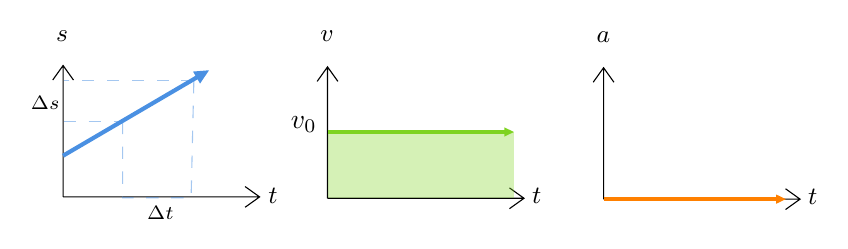
\begin{tikzpicture}[x=0.75pt,y=0.75pt,yscale=-1,xscale=1]
					%uncomment if require: \path (0,127); %set diagram left start at 0, and has height of 127
					
					%Shape: Axis 2D [id:dp4118351680260022] 
					\draw  (134.8,89.2) -- (229.47,89.2)(134.8,25.89) -- (134.8,89.2) -- cycle (222.47,84.2) -- (229.47,89.2) -- (222.47,94.2) (129.8,32.89) -- (134.8,25.89) -- (139.8,32.89)  ;
					%Shape: Axis 2D [id:dp42990141261180304] 
					\draw  (262.2,89.87) -- (356.87,89.87)(262.2,26.56) -- (262.2,89.87) -- cycle (349.87,84.87) -- (356.87,89.87) -- (349.87,94.87) (257.2,33.56) -- (262.2,26.56) -- (267.2,33.56)  ;
					%Shape: Axis 2D [id:dp1086498811664447] 
					\draw  (395.2,90.27) -- (489.87,90.27)(395.2,26.96) -- (395.2,90.27) -- cycle (482.87,85.27) -- (489.87,90.27) -- (482.87,95.27) (390.2,33.96) -- (395.2,26.96) -- (400.2,33.96)  ;
					%Straight Lines [id:da7462859480966277] 
					\draw [color={rgb, 255:red, 74; green, 144; blue, 226 }  ,draw opacity=0.5 ] [dash pattern={on 4.5pt off 4.5pt}]  (163.49,52.93) -- (163.49,89.6) -- (196.47,89.6) -- (197.8,33) ;
					%Straight Lines [id:da6875065720369709] 
					\draw [color={rgb, 255:red, 74; green, 144; blue, 226 }  ,draw opacity=1 ][line width=1.5]    (134.75,69.38) -- (201.65,30.2) ;
					\draw [shift={(205.11,28.18)}, rotate = 149.65] [fill={rgb, 255:red, 74; green, 144; blue, 226 }  ,fill opacity=1 ][line width=0.08]  [draw opacity=0] (6.97,-3.35) -- (0,0) -- (6.97,3.35) -- cycle    ;
					%Straight Lines [id:da2616373970106982] 
					\draw [color={rgb, 255:red, 74; green, 144; blue, 226 }  ,draw opacity=0.5 ] [dash pattern={on 4.5pt off 4.5pt}]  (197.8,33) -- (135.1,33) ;
					%Straight Lines [id:da6602255534348167] 
					\draw [color={rgb, 255:red, 74; green, 144; blue, 226 }  ,draw opacity=0.5 ] [dash pattern={on 4.5pt off 4.5pt}]  (135.13,52.93) -- (163.49,52.93) ;
					%Shape: Rectangle [id:dp41740211276161565] 
					\draw  [draw opacity=0][fill={rgb, 255:red, 126; green, 211; blue, 33 }  ,fill opacity=0.33 ] (262.2,57.92) -- (352,57.92) -- (352,89.87) -- (262.2,89.87) -- cycle ;
					%Straight Lines [id:da2292610893554068] 
					\draw [color={rgb, 255:red, 126; green, 211; blue, 33 }  ,draw opacity=1 ][line width=1.5]    (262.2,57.92) -- (348,57.92) ;
					\draw [shift={(352,57.92)}, rotate = 180] [fill={rgb, 255:red, 126; green, 211; blue, 33 }  ,fill opacity=1 ][line width=0.08]  [draw opacity=0] (4.64,-2.23) -- (0,0) -- (4.64,2.23) -- cycle    ;
					%Straight Lines [id:da3497236411867044] 
					\draw [color={orange}  ,draw opacity=1 ][line width=1.5]    (395.2,90.27) -- (479,90.27) ;
					\draw [shift={(483,90.27)}, rotate = 180] [fill={orange}  ,fill opacity=1 ][line width=0.08]  [draw opacity=0] (4.64,-2.23) -- (0,0) -- (4.64,2.23) -- cycle    ;
					
					% Text Node
					\draw (130.13,7.93) node [anchor=north west][inner sep=0.75pt]  [font=\small]  {$s$};
					% Text Node
					\draw (232.47,83.93) node [anchor=north west][inner sep=0.75pt]  [font=\small]  {$t$};
					% Text Node
					\draw (257.53,8) node [anchor=north west][inner sep=0.75pt]  [font=\small]  {$v$};
					% Text Node
					\draw (359.47,83.8) node [anchor=north west][inner sep=0.75pt]  [font=\small]  {$t$};
					% Text Node
					\draw (390.53,8.4) node [anchor=north west][inner sep=0.75pt]  [font=\small]  {$a$};
					% Text Node
					\draw (492.47,84.2) node [anchor=north west][inner sep=0.75pt]  [font=\small]  {$t$};
					% Text Node
					\draw (118,39.6) node [anchor=north west][inner sep=0.75pt]  [font=\scriptsize]  {$\Delta s$};
					% Text Node
					\draw (174,92.27) node [anchor=north west][inner sep=0.75pt]  [font=\scriptsize]  {$\Delta t$};
					% Text Node
					\draw (243.33,49.27) node [anchor=north west][inner sep=0.75pt]    {$v_{0}$};
					
					
				\end{tikzpicture}
			\end{figure}
		\end{grafik}
		
	\end{frame}
	
	\subsection{GLBB}
	
	\begin{frame}{Gerak Lurus Berubah Beraturan}
		\begin{defin}
			\footnotesize
			\justifying \noindent \textbf{Gerak lurus berubah beraturan} adalah gerakan pada lintasan garis lurus dengan kecepatan yang berubah secara beraturan dengan percepatan konstan ($\boldsymbol{a} = konstan$). \\ \noindent Jika $a > 0$, maka benda \textbf{dipercepat} (kecepatannya naik) dan untuk $a < 0$, benda \textbf{diperlambat} (kecepatannya turun).
		\end{defin}
		
			{\footnotesize
			\justifying \noindent Jika benda dengan kecepatan awal $v_0$ kecepatannya berubah menjadi $v$ dalam selang waktu $\Delta t (= t - t_0)$, maka \textbf{percepatannya} adalah
			\begin{equation}
				\boldsymbol{a} = \frac{\Delta \boldsymbol{v}}{\Delta t} = \frac{\boldsymbol{v} - \boldsymbol{v_0}}{t - t_0}
			\end{equation}}
			
			\begin{corr}[Pers. GLBB I]
				\footnotesize Memindahkan penyebut (ambil $t_0 = 0$) dan $v_0$ ke ruas yang lain pada Persamaan (B.2) memberikan suatu persamaan:
				
				\begin{equation}
					\boldsymbol{v} = \boldsymbol{v_0} + \boldsymbol{a} t
				\end{equation}
			\end{corr}
			
	\end{frame}

	\begin{frame}
		\begin{corr}[Pers. GLBB II]
			\small
			Mengintegralkan kedua ruas Persamaan (B.3) terhadap waktu memberikan kita suatu persamaan baru:
			
			\vspace{-1em}
			
			\begin{align}
				\int_{0}^{t} \boldsymbol{v} dt &= \int_{0}^{t}(\boldsymbol{v_0} + \boldsymbol{a}t) dt \notag \\
				\boldsymbol{s} - \boldsymbol{s_0} &= \boldsymbol{v_0}t + \frac{1}{2}\boldsymbol{a}t^2 \notag \\
				\boldsymbol{s} &= \boldsymbol{s_0} + \boldsymbol{v_0}t + \frac{1}{2}\boldsymbol{a}t^2
			\end{align}
			di mana $s$ dan $s_0$ secara berturut-turut adalah posisi pada waktu $t$ dan posisi awal (dan $\Delta \boldsymbol{s} = \boldsymbol{s} - \boldsymbol{s_0}$).
		\end{corr}
	\end{frame}
	
	\begin{frame}
		\begin{corr}[Pers. GLBB III]
			\small
			Dari Persamaan (B.4) kita dapatkan
			\begin{equation*}
				\Delta \boldsymbol{s} = (\boldsymbol{v_0} + \frac{1}{2}\boldsymbol{a}t)t
			\end{equation*}
			
			dan dengan mengkuadratkan kedua ruas Persamaan (B.3) kita dapatkan
			\begin{align}
				\boldsymbol{v}^2 &= \boldsymbol{v_0}^2 + 2\boldsymbol{v_0} \cdot \boldsymbol{a}t + \boldsymbol{a}^2 t^2 \notag \\
				&= \boldsymbol{v_0}^2 +2\boldsymbol{a}\underbrace{(\boldsymbol{v_0} + \frac{1}{2}\boldsymbol{a}t)t}_{\text{$= \Delta s$}} \notag \\
				\boldsymbol{v}^2 &= \boldsymbol{v_0}^2 + 2\boldsymbol{a} \cdot \Delta \boldsymbol{s}
			\end{align}
		\end{corr}
	\end{frame}
	
	\subsection{Gerak Vertikal}
	
	\begin{frame}{Gerak Vertikal}
		
		\begin{defin}
			\footnotesize
			\justifying \noindent \textbf{Gerak vertikal} adalah gerakan sepanjang sumbu vertikal. Di dekat permukaan Bumi, setiap benda dipengaruhi gravitasi Bumi sehingga memiliki percepatan ke arah pusat Bumi sebesar $\boldsymbol{a} = -\boldsymbol{g}$.\footnote{\tiny Tanda minus digunakan jika kita mengambil arah atas sebagai positif. Bagi kita yang berukuran kecil dibandingkan Bumi, arah ke pusat Bumi adalah ke "bawah" sehingga percepatan gravitasi Bumi arahnya ke "bawah", mengakibatkan tandanya menjadi negatif.} Dalam analisis, seringkali tanah dijadikan acuan ($y = 0$).
		\end{defin}
		
		
		\begin{corr}[Pers. GLBB I]
			\footnotesize \justifying Untuk menekankan bahwa gerakan terjadi pada sumbu-y, kita tambahkan subskrip $y$ pada kecepatan ($v_y$ dan $v_{y0}$) dan ganti $s$ dengan $y$. Percepatannya adalah $\boldsymbol{a} = -\boldsymbol{g}$. Jadi, persamaan geraknya adalah
			\begin{align}
				\boldsymbol{v_y} &= \boldsymbol{v_{y0}} - \boldsymbol{g}t\\
				\boldsymbol{y} &= \boldsymbol{y_0} + \boldsymbol{v_{y0}}t - \frac{1}{2} \boldsymbol{g}t^2\\
				\boldsymbol{v_y}^2 &= \boldsymbol{v_{y0}}^2 - 2\boldsymbol{g}\cdot\Delta\boldsymbol{y}
			\end{align}
		\end{corr}
		
%			\footnotesize \justifying  \noindent 
%			\noindent 
%		
%		\begin{corr}[Persamaan Gerak Vertikal]
%			{\scriptsize \justifying 
%		\end{corr}
%		
	\end{frame}
	
		\begin{frame}
		\begin{center}
			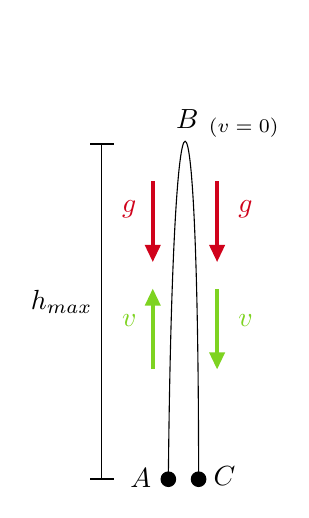
\begin{tikzpicture}[x=0.75pt,y=0.75pt,yscale=-1,xscale=1]
				%uncomment if require: \path (0,261); %set diagram left start at 0, and has height of 261
				
				%Shape: Ellipse [id:dp30878057149096994] 
				\draw  [fill={rgb, 255:red, 0; green, 0; blue, 0 }  ,fill opacity=1 ] (322,216.75) .. controls (322,214.81) and (323.57,213.24) .. (325.5,213.24) .. controls (327.44,213.24) and (329.01,214.81) .. (329.01,216.75) .. controls (329.01,218.68) and (327.44,220.25) .. (325.5,220.25) .. controls (323.57,220.25) and (322,218.68) .. (322,216.75) -- cycle ;
				%Curve Lines [id:da1745995487750911] 
				\draw    (325.5,216.75) .. controls (327.62,-0.54) and (340.11,-0.19) .. (340.08,216.75) ;
				%Shape: Ellipse [id:dp7130477090697445] 
				\draw  [fill={rgb, 255:red, 0; green, 0; blue, 0 }  ,fill opacity=1 ] (336.57,216.75) .. controls (336.57,214.81) and (338.14,213.24) .. (340.08,213.24) .. controls (342.01,213.24) and (343.58,214.81) .. (343.58,216.75) .. controls (343.58,218.68) and (342.01,220.25) .. (340.08,220.25) .. controls (338.14,220.25) and (336.57,218.68) .. (336.57,216.75) -- cycle ;
				%Straight Lines [id:da41901543924761575] 
				\draw [color={rgb, 255:red, 208; green, 2; blue, 27 }  ,draw opacity=1 ][line width=1.5]    (318,108) -- (318,93.45) -- (318,73.25) ;
				\draw [shift={(318,112)}, rotate = 270] [fill={rgb, 255:red, 208; green, 2; blue, 27 }  ,fill opacity=1 ][line width=0.08]  [draw opacity=0] (8.13,-3.9) -- (0,0) -- (8.13,3.9) -- cycle    ;
				%Straight Lines [id:da5237792005168593] 
				\draw [color={rgb, 255:red, 126; green, 211; blue, 33 }  ,draw opacity=1 ][line width=1.5]    (318,163.75) -- (318,129) ;
				\draw [shift={(318,125)}, rotate = 90] [fill={rgb, 255:red, 126; green, 211; blue, 33 }  ,fill opacity=1 ][line width=0.08]  [draw opacity=0] (8.13,-3.9) -- (0,0) -- (8.13,3.9) -- cycle    ;
				%Straight Lines [id:da2235781021974721] 
				\draw [color={rgb, 255:red, 208; green, 2; blue, 27 }  ,draw opacity=1 ][line width=1.5]    (349,108) -- (349,73.25) ;
				\draw [shift={(349,112)}, rotate = 270] [fill={rgb, 255:red, 208; green, 2; blue, 27 }  ,fill opacity=1 ][line width=0.08]  [draw opacity=0] (8.13,-3.9) -- (0,0) -- (8.13,3.9) -- cycle    ;
				%Straight Lines [id:da6674050395536943] 
				\draw [color={rgb, 255:red, 126; green, 211; blue, 33 }  ,draw opacity=1 ][line width=1.5]    (349,159.75) -- (349,125) ;
				\draw [shift={(349,163.75)}, rotate = 270] [fill={rgb, 255:red, 126; green, 211; blue, 33 }  ,fill opacity=1 ][line width=0.08]  [draw opacity=0] (8.13,-3.9) -- (0,0) -- (8.13,3.9) -- cycle    ;
				%Straight Lines [id:da7340915346785313] 
				\draw    (293.5,55.05) -- (293.5,216.75) ;
				\draw [shift={(293.5,216.75)}, rotate = 270] [color={rgb, 255:red, 0; green, 0; blue, 0 }  ][line width=0.75]    (0,5.59) -- (0,-5.59)   ;
				\draw [shift={(293.5,55.05)}, rotate = 270] [color={rgb, 255:red, 0; green, 0; blue, 0 }  ][line width=0.75]    (0,5.59) -- (0,-5.59)   ;
				
				% Text Node
				\draw (306,210.4) node [anchor=north west][inner sep=0.75pt]    {$A$};
				% Text Node
				\draw (346,209.4) node [anchor=north west][inner sep=0.75pt]    {$C$};
				% Text Node
				\draw (328,37.4) node [anchor=north west][inner sep=0.75pt]    {$B$};
				% Text Node
				\draw (333,41.4) node [anchor=north west][inner sep=0.75pt]  [font=\scriptsize]  {$\ \ \ ( v=0)$};
				% Text Node
				\draw (302,81.4) node [anchor=north west][inner sep=0.75pt]  [color={rgb, 255:red, 208; green, 2; blue, 27 }  ,opacity=1 ]  {$\boldsymbol{g}$};
				% Text Node
				\draw (358,81.4) node [anchor=north west][inner sep=0.75pt]  [color={rgb, 255:red, 208; green, 2; blue, 27 }  ,opacity=1 ]  {$\boldsymbol{g}$};
				% Text Node
				\draw (302,136.4) node [anchor=north west][inner sep=0.75pt]  [color={rgb, 255:red, 126; green, 211; blue, 33 }  ,opacity=1 ]  {$\boldsymbol{v}$};
				% Text Node
				\draw (358,136.4) node [anchor=north west][inner sep=0.75pt]  [color={rgb, 255:red, 126; green, 211; blue, 33 }  ,opacity=1 ]  {$\boldsymbol{v}$};
				% Text Node
				\draw (258,124.4) node [anchor=north west][inner sep=0.75pt]    {$h_{max}$};
				
				
			\end{tikzpicture}
		\end{center}
	
		\begin{corr}[Waktu untuk Mencapai Ketinggian Maksimum]
			\footnotesize Ketika berada di ketinggian maksimum, $\boldsymbol{v} = 0$. Substitusikan ke dalam Persamaan (B.6):
			\begin{equation}
				0 = {v_{y0}} - {g}t \quad \Longleftrightarrow \quad t = \frac{v_{y0}}{g}
			\end{equation}
		\end{corr}
	
	\end{frame}
	
	
	\begin{frame}
		\begin{corr}[Ketinggian Maksimum]
			\footnotesize Lagi, ketika berada di ketinggian maksimum, $\boldsymbol{v} = 0$. Perubahan ketinggiannya adalah $\Delta y = h_{max} - 0$. Substitusikan ke dalam Persamaan (B.8):
			\begin{equation}
				0^2 = v_{y0}^2 - 2g\cdot h_{max} \quad \Longleftrightarrow \quad h_{max} = \frac{v_{y0}^2}{2g}
			\end{equation}
		\end{corr}
	
		\begin{corr}[Waktu untuk Menumbuk Tanah]
			\footnotesize Ketika menumbuk tanah, $y = y_0$. Substitusikan ini ke dalam persamaan (B. 7):
			\begin{align}
				\coret{red}{y_0} &= \coret{red}{y_0} + v_{y0}t - \frac{1}{2} gt^2 \notag \\
				0 &= v_{y0}\coret{red}{t} - \frac{1}{2} gt^{\coret{red}{2}} \notag \\
				0 &= v_{y0} - \frac{1}{2} gt \notag \\
				t &= \frac{2v_{y0}}{g}
			\end{align}
		\end{corr}
	\end{frame}

	\begin{frame}
		\begin{corr}[Kecepatan ketika Menumbuk Tanah]
			\footnotesize Ketika menumbuk tanah, $y = y_0$ sehingga $y - y_0 = 0$, atau $\Delta y = 0$. Substitusikan ke persamaan (B.8):
			\begin{equation*}
				\boldsymbol{v}^2 = \boldsymbol{v_{y0}}^2 - 2 \boldsymbol{g} \cdot 0 \quad \Longleftrightarrow \quad v^2 = v_{y0}^2
			\end{equation*}
			Karena arah kecepatan awal dan akhir berlawanan, maka $v = - v_{y0}$.
		\end{corr}
	\end{frame}
	
	
	\subsection{Gerak pada Bidang Miring}
	
	\begin{frame}
		content...
	\end{frame}
	
	\section{Gerak Parabola}
	
	\begin{frame}{Gerak Parabola}
		content...
	\end{frame}
	
	\section{Gerak Melingkar Beraturan}
	
	\begin{frame}{Gerak Melingkar Beraturan}
		content...
	\end{frame}

	\section{}
	
	\begin{frame}
		
		\begin{center}
			\textbf{\LARGErrr Terima Kasih}
		\end{center}
		
	\end{frame}
	
\end{document}